\documentclass[11pt]{article}

\usepackage[utf8]{inputenc}
\usepackage[T1]{fontenc}
\usepackage{lmodern}
\usepackage[margin=1in]{geometry}
\usepackage{graphicx}
\usepackage{booktabs}
\usepackage{array}
\usepackage{amsmath}
\usepackage{hyperref}
\usepackage{xcolor}

\hypersetup{
  colorlinks=true,
  linkcolor=blue!50!black,
  citecolor=blue!50!black,
  urlcolor=blue!60!black
}

\title{Blocking Cross-Session Token Splicing in OAuth Token Exchange\\
\large A Session-Bound Capability Chain for Delegation Integrity}
\author{CS5321 Team 35}
\date{April 2026}

\begin{document}
\maketitle

\begin{abstract}
OAuth 2.0 token exchange is widely used to propagate user context across service-to-service calls, but the specification does not force a Security Token Service (STS) to verify the full continuity of a delegation path. In this project we show that a vulnerable STS can accept a forged delegation chain when an attacker combines a stolen delegated token with their own actor token, creating a path that never existed in the real system. We implement this cross-session token splicing attack in a compact Python prototype and then design a defense that combines a direct path-integrity check with a session-bound capability chain inspired by Stateless Internet Flow Filter (SIFF)-style path validation. The resulting secure STS binds every delegation hop to a shared session identifier, validates a signed chain of capabilities, prevents scope expansion, and rejects replayed requests. Across 17 unit tests, the secure design blocks token splicing, replay, tampering, and scope-escalation attempts while adding only sub-millisecond overhead in our local measurements.
\end{abstract}

\section{Introduction}
Modern distributed systems often rely on delegated credentials: a front-end service acts for a user, obtains a token, and later exchanges it so downstream services can continue the request with narrower permissions. This pattern is convenient, but it creates a subtle integrity requirement: every hop in the delegation chain must be continuous. If that continuity is not checked, a token exchange endpoint may validate each token in isolation while still accepting a forged path.

This report studies that exact problem for an RFC 8693-style STS. Our baseline implementation uses signed JWTs and nested \texttt{act} claims to represent delegation history. We show that the baseline is vulnerable to a cross-session token splicing attack: the attacker steals a token intended for another agent and pairs it with their own valid token as the actor, causing the STS to mint a new token on behalf of the victim user. We then present a defense with two layers:

\begin{itemize}
  \item a direct path-integrity check that verifies the caller is the agent the stolen token was actually issued to; and
  \item a session-bound capability chain that records each delegation hop as a signed capability and binds all hops to one session identifier.
\end{itemize}

The result is a concise but complete prototype that makes the attack concrete, demonstrates why individual signature checks are not enough, and shows how delegation-path validation can be enforced with low overhead.

\section{System Model and Baseline Flow}
\subsection{Actors and tokens}
Our prototype models a user, a sequence of agents, and a shared STS. The STS issues JWTs signed with HS256. Each token contains four core fields:

\begin{itemize}
  \item \texttt{sub}: the original user identity,
  \item \texttt{aud}: the agent the token is currently intended for,
  \item \texttt{act}: a nested actor chain that records the current holder and prior holders,
  \item \texttt{scope}: the permissions carried by the token.
\end{itemize}

In the secure design, tokens also carry a \texttt{session\_id} so that all delegation artifacts from the same request flow can be linked together.

\subsection{Normal delegation workflow}
The expected workflow is straightforward. Alice authenticates to Agent A. Agent A obtains an initial grant from the STS, then exchanges that token for a downstream token intended for Agent B with narrower scope. Figure~\ref{fig:baseline} illustrates this baseline flow and the resulting token state.

\begin{figure}[htbp]
  \centering
  
\includegraphics[width=\linewidth]{01-system-baseline-normal-delegation.svg.png}
  \caption{Normal delegation flow in the baseline system. The STS first issues a token for Agent A, which is then exchanged for a narrower token for Agent B.}
  \label{fig:baseline}
\end{figure}

For a valid exchange, the token being presented must have been issued to the agent now presenting it. In our setting, that continuity requirement can be expressed as:

\[
\texttt{subject\_token.aud = actor\_token.act.sub}
\]

If this invariant is not enforced, the STS can be tricked into stitching together unrelated pieces of delegation state.

\section{Attack on the Vulnerable STS}
\subsection{Root cause}
The vulnerable baseline verifies token signatures and checks that the \texttt{caller} matches the current actor recorded in the actor token. However, it does \emph{not} verify that the subject token was actually issued to that actor. In other words, it never checks whether \texttt{subject\_token.aud} matches \texttt{actor\_token.act.sub}. This omission is enough to break delegation continuity.

\subsection{Threat model}
We assume the attacker can:

\begin{itemize}
  \item obtain their own legitimately issued token from the STS,
  \item steal a delegated token that was issued to some other agent,
  \item call the token exchange endpoint as themselves.
\end{itemize}

We do \emph{not} assume the attacker can forge JWT signatures, break cryptography, or impersonate arbitrary agents. The attack succeeds purely because the STS fails to confirm that the delegation path is continuous.

\subsection{Token splicing attack}
The attack proceeds in two stages. First, the legitimate system creates a path \texttt{Alice -> Agent A -> Agent B}. Second, the attacker steals Agent B's token and pairs it with their own actor token. Since the vulnerable STS only checks that the attacker is indeed the caller represented by their own token, it issues a new token that appears to extend Alice's delegation path to the attacker.

Figure~\ref{fig:attack} shows the attack visually. The stolen token and attacker-controlled actor token meet at the splice point. Because path continuity is never checked, the vulnerable STS accepts the request and returns a forged token.

\begin{figure}[htbp]
  \centering
  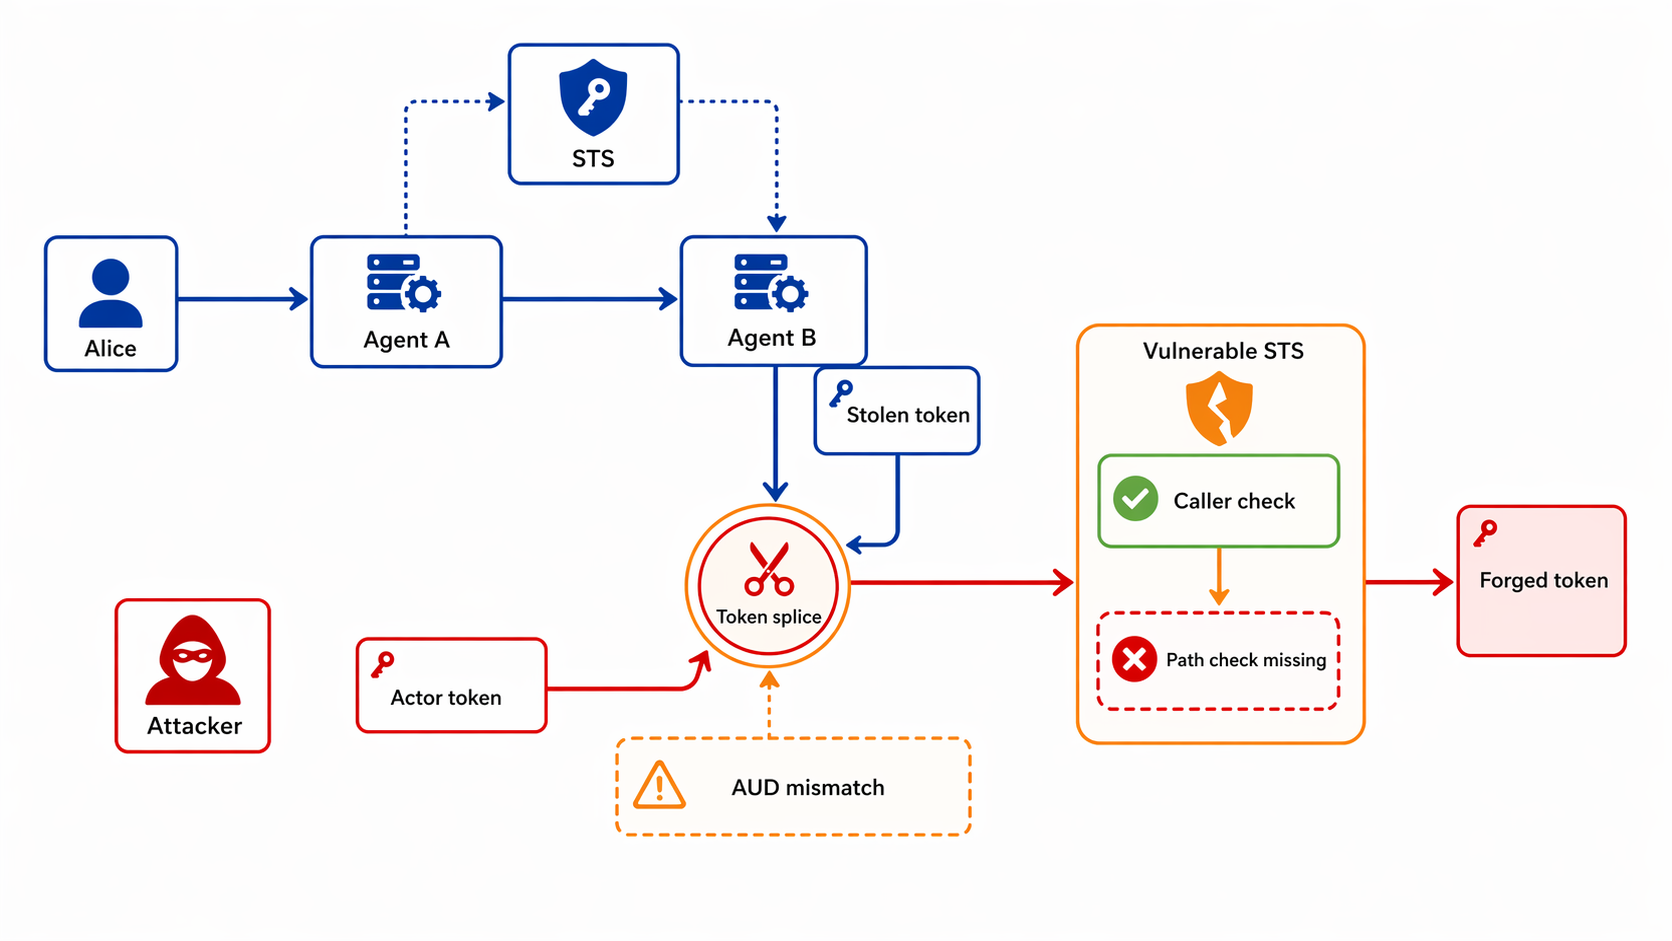
\includegraphics[width=\linewidth]{02-vulnerability-token-splicing-attack.png}
  \caption{Cross-session token splicing against the vulnerable STS. A stolen delegated token is combined with the attacker's own actor token to create a forged path.}
  \label{fig:attack}
\end{figure}

In our demo, the attacker receives a token with:

\begin{itemize}
  \item \texttt{sub = alice},
  \item \texttt{aud = attacker},
  \item scope \texttt{[A, B, C]}, even though Agent B only held \texttt{[A, B]}.
\end{itemize}

This demonstrates two failures at once: forged delegation history and scope escalation. Most importantly, the path \texttt{Alice -> Agent A -> Agent B -> Attacker} never existed in the actual system.

\section{Defense: Session-Bound Capability Chain}
\subsection{Layer 1: path-integrity check}
The most direct fix is to enforce the missing invariant:

\[
\texttt{subject\_token.aud = actor\_token.act.sub}
\]

This check ensures the token being exchanged was actually issued to the entity presenting it. In the splicing attack, the subject token was issued to Agent B while the actor token identifies the attacker, so the request is rejected immediately.

\subsection{Layer 2: signed capability chain}
The direct check closes the baseline splice, but we additionally wanted a mechanism that records the full path in a cryptographically verifiable form. Inspired by SIFF, we attach a signed capability to each hop. Every capability contains:

\begin{itemize}
  \item a shared \texttt{session\_id},
  \item the hop number,
  \item the \texttt{from} and \texttt{to} principals,
  \item the granted scope,
  \item issuance and expiry times,
  \item a nonce used for replay prevention.
\end{itemize}

Each capability is signed by the STS using HMAC-SHA256. On every exchange, the caller must present the full capability chain accumulated so far. The secure STS validates:

\begin{itemize}
  \item signature correctness for every capability,
  \item capability freshness,
  \item session continuity through one shared \texttt{session\_id},
  \item contiguous hop numbering,
  \item path continuity where \texttt{chain[i-1].to = chain[i].from},
  \item nonce freshness for the last hop,
  \item scope monotonicity so permissions can only stay the same or shrink.
\end{itemize}

Figure~\ref{fig:defense} summarizes the secure validation pipeline.

\begin{figure}[htbp]
  \centering
  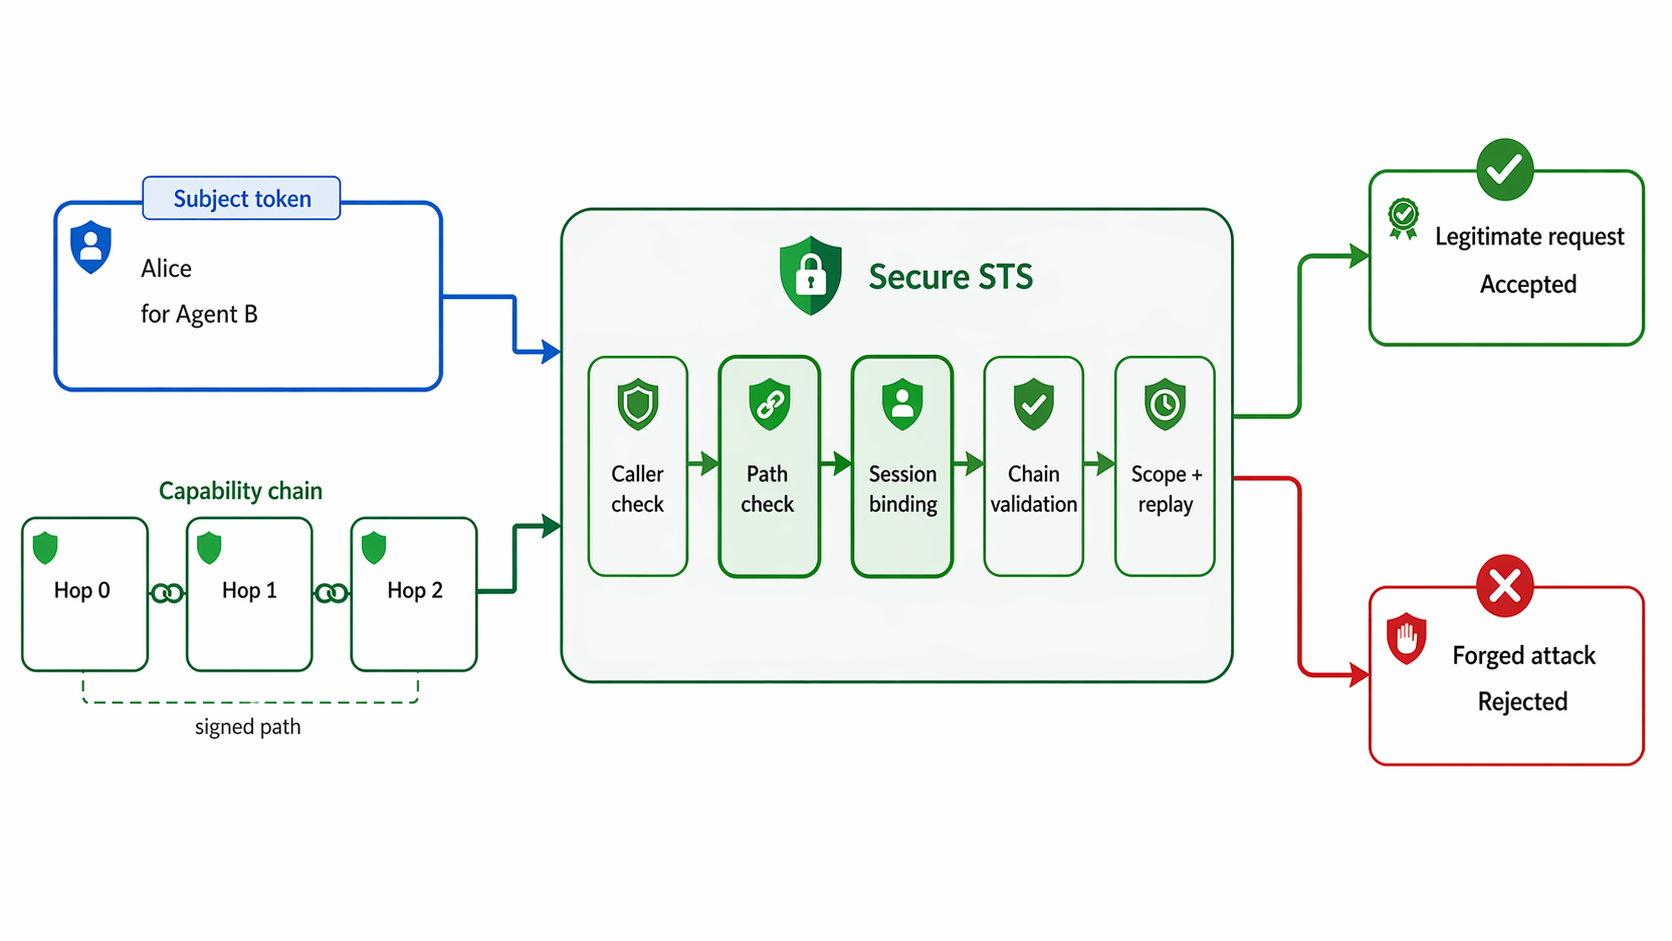
\includegraphics[width=\linewidth]{03-defense-secure-sts-validation.png}
  \caption{Secure STS validation pipeline. A request is accepted only if caller identity, path integrity, session binding, capability-chain validation, and scope/replay checks all succeed.}
  \label{fig:defense}
\end{figure}

\subsection{Why the chain prevents cross-session splicing}
The key idea is that capability chains are session-bound and hop-complete. An attacker who was never part of Alice's delegation flow never receives the signed capabilities for that session. Even if they steal one delegated token, they cannot fabricate the missing chain entries or change the session identifier without breaking the capability signature. This turns the informal delegation path into an explicit cryptographic object that the STS can validate end-to-end.

\section{Implementation}
We implemented the project in Python with two STS variants:

\begin{itemize}
  \item \texttt{sts/vulnerable\_sts.py} models the insecure exchange logic.
  \item \texttt{sts/secure\_sts.py} adds session binding, capability validation, replay prevention, and scope checks.
\end{itemize}

The supporting files are intentionally small and focused. \texttt{utils/token\_utils.py} handles JWT signing and capability signatures, while \texttt{agent.py} models baseline and secure agents. Two demo scripts replay the vulnerable and secure scenarios, and the test suite exercises both positive and negative cases.

The secure implementation uses a fresh random \texttt{session\_id} at \texttt{initial\_grant()} time, appends one signed capability per delegation hop, and stores seen nonces in memory to reject replayed requests. This is enough to capture the security logic clearly, even though it simplifies a full production OAuth deployment.

\section{Evaluation}
\subsection{Functional security results}
Our evaluation combines live demos with unit tests. The vulnerable demo confirms that token splicing succeeds on the baseline STS. The secure demo shows that the defended STS blocks four concrete attack classes:

\begin{table}[htbp]
  \centering
  \begin{tabular}{>{\raggedright\arraybackslash}p{0.33\linewidth} >{\raggedright\arraybackslash}p{0.57\linewidth}}
    \toprule
    Attack & Rejection reason in the secure STS \\
    \midrule
    Token splicing & Path-integrity check fails because \texttt{aud} does not match the presenting actor \\
    Replay of capability chain & Last-hop nonce already marked as used \\
    Scope escalation & Requested scopes are not a subset of the previous hop's scope \\
    Tampered capability & HMAC signature over the capability no longer verifies \\
    \bottomrule
  \end{tabular}
  \caption{Observed attack outcomes in the secure demo.}
  \label{tab:blocked}
\end{table}

\subsection{Unit-test coverage}
The repository contains 17 unit tests, all passing in our local run. Table~\ref{tab:tests} groups them by security objective.

\begin{table}[htbp]
  \centering
  \begin{tabular}{l c p{0.48\linewidth}}
    \toprule
    Category & Count & What is verified \\
    \midrule
    Legitimate flow & 5 & Initial grant format, session propagation, scope narrowing, actor-chain growth, chain depth \\
    Path integrity & 3 & Token splicing rejection, wrong-session rejection, missing \texttt{session\_id} rejection \\
    Replay prevention & 1 & Replayed nonce detection \\
    Chain tampering & 4 & Invalid signature, tampered session identifier, non-contiguous hops, broken path continuity \\
    Scope enforcement & 2 & Scope escalation blocked, subset scope accepted \\
    Vulnerable baseline & 1 & Splicing still succeeds when the baseline STS is used \\
    \midrule
    Total & 17 & All tests passed \\
    \bottomrule
  \end{tabular}
  \caption{Test coverage of the secure design.}
  \label{tab:tests}
\end{table}

\subsection{Performance overhead}
We also measured the secure exchange cost over 200 rounds for delegation depths from 1 to 5. The results are shown in Table~\ref{tab:perf}.

\begin{table}[htbp]
  \centering
  \begin{tabular}{c c c}
    \toprule
    Delegation depth & Average exchange latency (ms) & Approximate chain size (chars) \\
    \midrule
    1 & 0.038 & 600 \\
    2 & 0.079 & 902 \\
    3 & 0.123 & 1204 \\
    4 & 0.191 & 1506 \\
    5 & 0.233 & 1808 \\
    \bottomrule
  \end{tabular}
  \caption{Observed secure-STS overhead on a local machine.}
  \label{tab:perf}
\end{table}

Two trends are clear. First, latency increases roughly linearly with chain depth because each hop adds one more signed capability to validate. Second, chain size also grows linearly because the full signed path is carried forward. In this prototype the absolute overhead remains very small: even at depth 5, average validation time stays well below one millisecond.

\section{Discussion and Limitations}
The project demonstrates the core integrity issue clearly, but it intentionally abstracts away several production concerns.

\begin{itemize}
  \item The prototype uses a shared HMAC secret instead of asymmetric signatures and key rotation.
  \item Replay prevention stores seen nonces in local memory, which would need a distributed design in a real multi-instance deployment.
  \item The capability chain grows linearly with delegation depth. A production system might compress prior hops into a signed accumulator or hash commitment.
  \item The model focuses on delegation integrity inside the STS rather than the full OAuth ecosystem, such as client authentication, revocation, or transport-layer trust.
\end{itemize}

Even with these simplifications, the core result is meaningful: verifying token signatures is not enough if the exchange service does not also verify that the presented artifacts belong to one continuous delegation session.

\section{Conclusion}
This project shows that a vulnerable RFC 8693-style STS can be compromised without breaking cryptography. By combining a stolen delegated token with a legitimate actor token from a different session, an attacker can splice themselves into a delegation path that never existed and receive a forged token on behalf of another user.

Our defense addresses the problem in a principled way. A direct path-integrity check blocks the immediate splice condition, while a session-bound capability chain turns each delegation hop into a signed, replay-resistant, session-consistent record. The resulting secure STS blocks all attack variants we tested and does so with low overhead. The broader lesson is that delegated authorization requires path integrity, not just token validity.

\begin{thebibliography}{9}

\bibitem{rfc8693}
M. B. Jones, A. Nadalin, B. Campbell, J. Bradley, and C. Mortimore,
\emph{OAuth 2.0 Token Exchange},
RFC 8693, January 2020.
\url{https://www.rfc-editor.org/rfc/rfc8693}

\bibitem{rfc7519}
M. B. Jones, J. Bradley, and N. Sakimura,
\emph{JSON Web Token (JWT)},
RFC 7519, May 2015.
\url{https://www.rfc-editor.org/rfc/rfc7519}

\bibitem{siff}
A. Yaar, A. Perrig, and D. Song,
\emph{SIFF: A Stateless Internet Flow Filter to Mitigate DDoS Flooding Attacks}.
\url{https://users.ece.cmu.edu/~dawnsong/papers/siff.pdf}

\end{thebibliography}

\end{document}
